%!TEX root = ../report.tex
\section{Taktik}

\subsection{Begriffe \& Systematik}
\begin{description}
  \item[Taktik] ist ein System von Handlungsplänen und Entscheidungsalternativen, das Trainings- und Wettkampfverhalten so zu regulieren gestattet, dass ein optimaler sportlicher Erfolg möglich wird.
  \item[Strategie] ist über längere Zeit gesehene Taktik.
  \item[Taktisches Verhalten] bedeutet eine Situation mit einer Handlung zu beantworten
  \item[Taktisch entscheiden] bedeutet in einer Situation aus einer Menge aus Alternativen einen Handlungsplan auswählen. Es existieren verschiedene Kopplungsmodelle dieses Auswahlverfahrens: Feste Assoziation (eine Situation impliziert genau eine Handlung), Auswahl aus Alternativen (eine Situation kann eine Gruppe von Handlungen implizieren), Vorsatzhandlungen (es existiert nur eine Handlungsalternative).
\end{description}
\begin{figure}[H]
  \begin{flushleft}
    \textbf{Systematisierung nach Zeit}
  \end{flushleft}
  \centering
  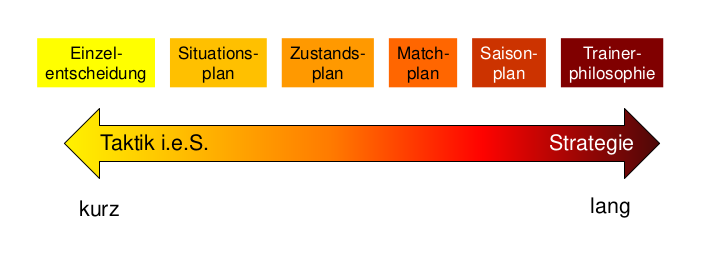
\includegraphics[width=.7\textwidth]{pictures/taktik_systematisierung.png}
  \caption{Systematisierung von Taktik nach Zeit}
\end{figure}
\paragraph{Systematisierung nach \# beteiligter Spieler} Taktik kann abhängig von der Anzahl der Spieler eingeteilt werden. Teilbereiche sind dann Mannschaftstaktik, Gruppentaktik und Individualtaktik.
\paragraph{Systematisierung nach Spielsituation} Mögliche Varianten sind Standardsituation, Offensivtaktik, Defensivtaktik, Übergangsphasen
\paragraph{Systematisierung nach Trainingszielen}
\begin{itemize}
  \item Taktische Kenntnisse: Wissensbestände, deklaratives Wissen
  \item Taktische Fähigkeiten: Situationsübergreifende taktische Handlungskompetenz: Wahrnehmung, Entscheidung, Ausführung
  \item Taktische Fertigkeiten: Angemessene und erfolgreiche Antworthandlungen (Individuell, teilkollektiv und kollektiv)
\end{itemize}
\paragraph{Taktische Handlungsphasen (nach Heckhausen)}
\begin{enumerate}
  \item Prädezisionale Phase: Wählen/ Entscheiden
  \item Präaktionale Phase: Planen/ Abschirmen
  \item Aktionale Phase: Ausführen
  \item Postaktionale Phase: Vergleichen/ Bewerten
\end{enumerate}
\begin{figure}[H]
  \begin{flushleft}
    \textbf{Phasenstruktur taktischen Handelns (nach Mahlo)}
  \end{flushleft}
  \centering
  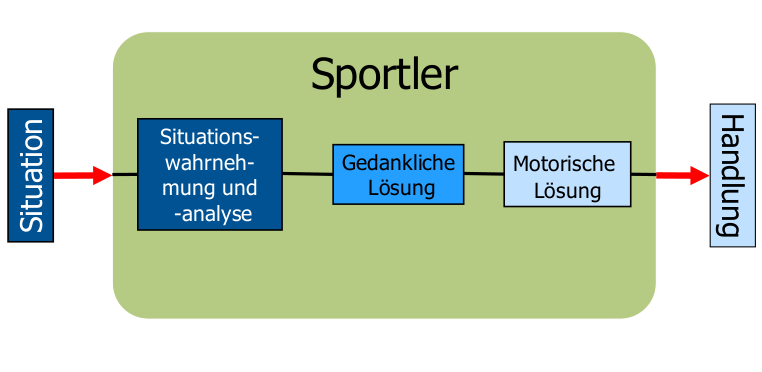
\includegraphics[width=.7\textwidth]{pictures/taktik_phasenstruktur_des_handelns.png}
\end{figure}
Probleme dieses Ansatzes:
\begin{itemize}
  \item Werden die Phasen vollständig durchlaufen?
  \item Werden die Phasen nacheinander druchlaufen?
  \item Entscheidungen werden bewusst getroffen
\end{itemize}
\paragraph{Fehlerquellen bei taktischen Entscheidungen} Taktische Fehlentscheidungen können durch alle 3 Phasen enstehen. Falsche Situationswahrnehmung und -analyse (sensorische Probleme), Inkorrekte gedankliche Lösungen (Wahl der falschen Alternative, Menge an Vorerfahrung, akt. Einflüsse) und eine mangelnde motorische Umsetzung (Fehleinschätzung der Fähigkeiten, situative Umstände)
\paragraph{Entscheidungsmodelle der Psychologie}
\begin{itemize}
  \item Zufallsentscheidung
  \item Heuristische Entscheidung
  \item Rational-Choice Entscheidung: viele Theorien, z.B.\ Erwartungs-mal-Wert-Therie (Probleme: alle Alternativen, Werte \& Wahrscheinlichkeiten bekannt?)
\end{itemize}
\paragraph{Aktuelle Theorien - Top-down \& Bottom-up Prozesse}
\begin{description}
  \item[Top-down Prozesse] Kognitionsgesteuerte, verbalisierbare Erwartungs- und Zielbildungsprozesse (Wenn A dann B)
  \item[Bottom-up Prozesse] Wahrnehmungs- gesteuerte, nicht verbalisierbare Wahrnehmungs- Handlungsprozesse. (Reaktionen)
\end{description}
Mögliche Zusammenspiele der beiden Prozesse:\\
\begin{minipage}{0.1\textwidth}
  
\includegraphics[width=\textwidth]{pictures/taktik_top-down_bottom-up.png}
\end{minipage}
\begin{minipage}{0.9\textwidth}
  \begin{itemize}
    \item Selektion: Nur je ein Typ aktiv (Vorsatzhandlungen)
    \item Konkurrenz: 1 Typ dominiert, i.d.R.\ Top-down (einfache Situationen)
    \item Kooperation: beide in gleiche Richtung (komplexe Situationen)
    \item Korrektur: Wahrnehmung korrigiert Entscheidung
  \end{itemize}
\end{minipage}
Top-down Prozesse sind explizit lehrbar, Bottom-up nicht/nur implizit. Lehren von Top-down Prozessen beinhaltet taktisches Wissen, Spielsysteme, Standardsituationen und Vorsatzhandlungen. Implizites Botto-up Training beinhaltet das Verhalten im Raum, das Erkennen von Optionen, Lesen des Gegners und die Lösung von Situationen.

\subsection{Determinanten}
\begin{figure}[H]
  \centering
  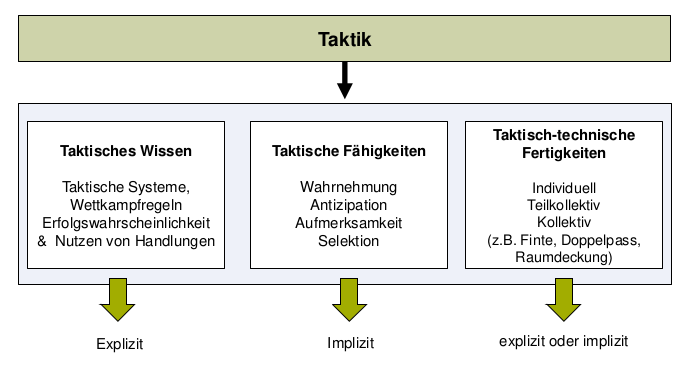
\includegraphics[width=.7\textwidth]{pictures/taktik_determinanten.png}
\end{figure}

\subsection{Trainingsmethoden}

\subsection{Trainingsinhalte}

\subsection{Anwendung}

\subsection{Diagnostik}

\subsection{Zusammenfassung}
